%ju 28-Mai-22 FM_U07_gemischte_Schaltung_Loesung.tex
\section{gemischte Schaltung Übung
7}\label{gemischte-schaltung-uebung-7}

\textbf{Aufgabe 1}

\begin{figure}[!ht]% hier: !ht
\centering
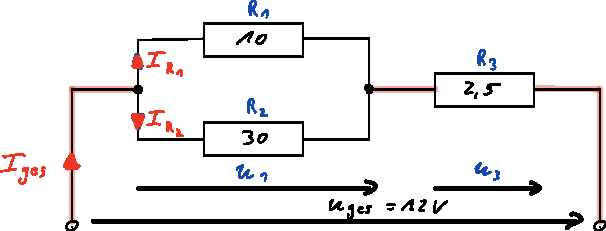
\includegraphics[width=0.6\textwidth]{images/Skizze/25_FM_Nr7_gemischte_Schaltung_A1.pdf}
\caption{FM Nr7 gemischte Schaltung A1}
%\label{fig:}%% anpassen
\end{figure}

\lstset{language=Python}% C, TeX, Bash, Python 
\begin{lstlisting}[
	%caption={}, label={code:}%% anpassen
][language=Python]
# geg: Mathebuch S. 82 Aufgabe 6 Schaltung
R_1 = 10 Ohm
R_2 = 30 Ohm
R_3 = 2,5 Ohm
U_ges = 12 V
# ges: R_I, R_ges, I_ges, U_1, U_3, I_R_1, I_R_2
# Formel:
R_I = 1/(1/R_1 + 1/R_2)
R_ges = R_I + R_3
I_ges = U_ges/R_ges
U_1 = R_I x I_ges
U_3 = R_3 x I_ges
I_R_1 = U_1/R_1
I_R_2 = U_1/R_2
# Lösung:
R_I = 7,5 Ohm
R_ges = 10,0 Ohm
I_ges = 1,2 A
U_1 = 9,0 V
U_3 = 3,0 V
I_R_1 = 0,9 A
I_R_2 = 0,3 A
\end{lstlisting}

\newpage

\textbf{Aufgabe 2}

\begin{figure}[!ht]% hier: !ht
\centering
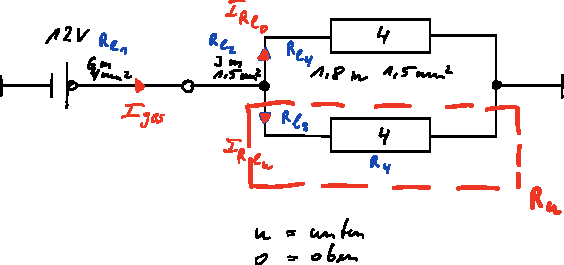
\includegraphics[width=0.6\textwidth]{images/Skizze/25_FM_Nr7_gemischte_Schaltung_A2.pdf}
\caption{FM Nr7 gemischte Schaltung A2}
%\label{fig:}%% anpassen
\end{figure}

\lstset{language=Python}% C, TeX, Bash, Python 
\begin{lstlisting}[
	%caption={}, label={code:}%% anpassen
][language=Python]
# geg: Schaltung
U_ges = 12 V
l_1 = 6 m
A_1 = 4 mm^2
l_2 = 3 m
A_2 = 1,5 mm^2
l_3 = 1,8 m
A_3 = 1,5 mm^2
R_4 = 4 Ohm
p = 0,0178 Kupfer ohm x mm^2 / m 
# ges: U_v_Leitung
# Formel:
R_l_1 = p x l_1 / A_1
R_l_2 = p x l_2 / A_2
R_l_3 = p x l_3 / A_3
R_u = R_l_3 + R_4 (R_o = R_u)
R_II = R_u/2
R_ges = R_l_1 + R_l_2 + R_II
I_ges = U_ges/R_ges
U_v_R_l_3 = R_l_3 x I_R_l_3 -> U_v_R_l_3 = (R_l_3 x I_ges)/2
# Lösung:
R_l_1 = 0,0267 Ohm
R_l_2 = 0,0356 Ohm
R_l_3 = 0,0214 Ohm
R_u = 4,0214 Ohm
R_l_1 = 0,0267 Ohm
R_II = 2,0107 Ohm
R_ges = 2,073 Ohm
I_ges = 5,7888 A
U_v_R_l_3 = 0,0618 V
\end{lstlisting}

\newpage

\textbf{Aufgabe 3}

\begin{figure}[!ht]% hier: !ht
\centering
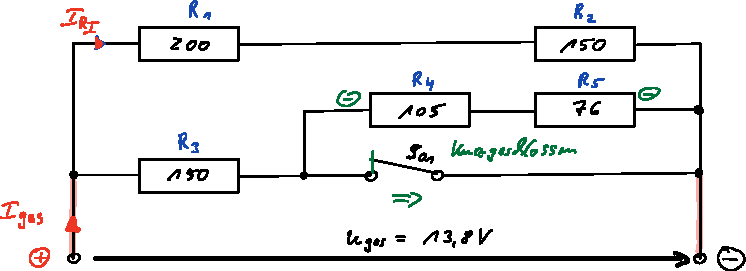
\includegraphics[width=0.6\textwidth]{images/Skizze/25_FM_Nr7_gemischte_Schaltung_A3.pdf}
\caption{FM Nr7 gemischte Schaltung A3}
%\label{fig:}%% anpassen
\end{figure}

\lstset{language=Python}% C, TeX, Bash, Python 
\begin{lstlisting}[
	%caption={}, label={code:}%% anpassen
][language=Python]
# geg: Schaltung
R_1 = 200 Ohm
R_2 = 150 Ohm
R_3 = 150 Ohm
R_4 = 105 Ohm
R_5 = 76 Ohm
U_ges = 13,8 V
# Formel:
# 3,1) ges: R_I, R_II, R_ges_1, R_ges_2, R_delta
R_I = R_1 + R_2
R_II = R_3 + R_4 + R_5 (Schalter offen)
R_ges_1 = 1/(1/R_I + 1/R_II) (Schalter offen)
R_ges_2 = 1/(1/R_II + 1/R_3) (Schalter zu)
R_delta = R_ges_1 - R_ges_2
Gesamtwiderstand ändert sich
# 3,3) ges: I_R_3
I_R_3 = U_ges/R_II (Schalter offen)
# 3,4) ges: U_S_01
U_S_01 = (R_4 + R_5) x I_R_3 (Schalter offen)
# 3,5) ges: I_R_1
I_R_1 = U_ges/R_I
Strom bleibt immer gleich, egal ob Schalter auf/zu
# Lösung:
R_I = 350 Ohm
R_II = 331 Ohm
R_ges_1 = 170,1175 Ohm
R_ges_2 = 103,2225 Ohm
R_delta = 66,895 Ohm
I_R_3 = 0,0417 A
U_S_01 = 7,5462 V
I_R_1 = 0,0394 A
\end{lstlisting}

\newpage

\textbf{Aufgabe 4}

\begin{figure}[!ht]% hier: !ht
\centering
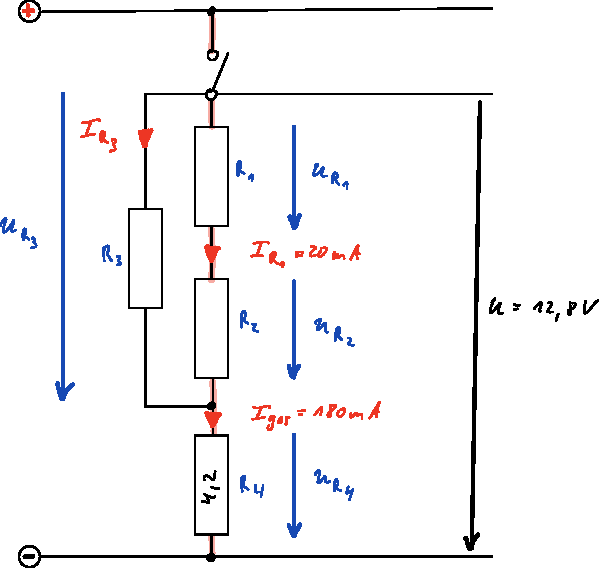
\includegraphics[width=0.6\textwidth]{images/Skizze/25_FM_Nr7_gemischte_Schaltung_A4.pdf}
\caption{FM Nr7 gemischte Schaltung A4}
%\label{fig:}%% anpassen
\end{figure}

\lstset{language=Python}% C, TeX, Bash, Python 
\begin{lstlisting}[
	%caption={}, label={code:}%% anpassen
][language=Python]
# geg: Schaltung
R_4 = 4,2 Ohm
U_ges = 12,8 V
U_R_2 = 1,65 V
I_R_1 = 0,02 A = 20 mA
I_ges = 0,18 A = 180 mA
# ges: R_2, U_R_4, R_1, R_3
# Formel:
R_2 = U_R_2/I_R_1
U_R_4 = R_4 x I_ges
R_1 = U_R_1/I_R_1 -> R_1 = (U_ges - U_R_2 - U_R_4)/I_R_1
R_3 = U_R_3/I_R_3 -> R_3 = (U_ges - U_R_4)/(I_ges - I_R_1)
# Lösung:
R_2 = 82,5 Ohm
U_R_4 = 0,756 V
R_1 = 519,7 Ohm
R_3 = 75,275 Ohm
\end{lstlisting}
